% !TeX program = lualatex -shell-escape
\documentclass{beamer}

\usepackage{focs-slides}
\usepackage{graphicx}
\usepackage[cache=false]{minted}
\usepackage{multicol}

\setminted{
	linenos,
	breaklines,
	fontsize=\footnotesize,
	tabsize=4
}
\setmintedinline{
	fontsize=\footnotesize
}

\usepackage[utf8]{inputenc}
\usepackage{tcolorbox}
\tcbuselibrary{minted,skins}

\definecolor{bill}{RGB}{0,0,0}
\definecolor{numC}{RGB}{220,220,220}

\newtcblisting{mycodetiny}{
	listing engine=minted,
	minted style=perldoc,
	minted language=python,
	minted options={fontsize=\scriptsize,linenos,numbersep=-7mm},
	%colback=bill,
	%colframe=bill,
	listing only,
	left=-5mm,
	enhanced,
	overlay={\begin{tcbclipinterior}\fill[numC](frame.south west)rectangle([xshift=5mm]frame.north west);\end{tcbclipinterior}}
}

\usefonttheme[onlymath]{serif}

\title{RecomMuse}
\author{Kantaphat Leelakunwet, Choo Lee Wen, Arsen Aghayan, Ibrahim Daurenov}
\date{Summer 2025}
\course{ECE472}

% bibliography file
\addbibresource{project.bib}

\definecolor{darkblue}{HTML}{6666dd} 
\definecolor{darkslategray}{HTML}{2f4f4f} 
%\colortheme{green!42!black}
%\colortheme{orange!85!black}
%\colortheme{darkblue}
% \colortheme{pink!80!black}
\colortheme{orange!85!white!90!black}
% \colortheme{yellow!100!white!90!black}
% \colortheme{darkslategray}

\begin{document}

\maketitle

% \begin{frame}{Goal}

% \begin{center}
%     RecomMuse - Where Data Meets Your Playlist
    
%     \vspace{0.5cm}
    
%     Traditional platforms recommend similar songs.

%     How do we help listeners discover deeper connections?

%     \vspace{0.5cm}

%     Using Hadoop, Spark, and Drill, we built a system that doesn't just play music... it understands musical relationships.
    
% \end{center}

% \end{frame}

% table of contents
\toc{enum}
% \toc{mindmap}

\section{Data Processing}

\begin{frame}{Motivation}

    \textbf{Challenge}
    \begin{itemize}
        \item One million tiny HDF5 files
        \item RAM overload on namenode
    \end{itemize}
    
    \textbf{Solution}
    \begin{itemize}
        \item Use JHDF to extract relevant features
        \item Compact small files into a larger one
    \end{itemize}

    \textbf{JHDF (Java HDF5 Library)}
    \begin{itemize}
        \item Pure Java. Easy integration with JVM based project.
        \item No use of JNI. Avoid issues with calling native code from JVM.
        \item It provides fast file access and reading is parallelized.
    \end{itemize}
    
\end{frame}

\begin{frame}{Avro Compaction}

    \begin{itemize}
        \item Tailored Avro schema - keeping only essential features such as timbre, tempo, etc for year prediction and drill queries.
        \item Snappy compression
        \item Processed files alphabetically - A through Z
        \item Each letter batch took about 25-30 minutes - producing tidy 66 MB Avro files
        \item Finally merged everything into one single 1.7 GB file.
        \item \textbf{99.4\%} Storage Reduction (Original is 286.6 GB)
        \item You could analyze it on a single commodity hardware easily.
    \end{itemize}

\end{frame}

\section{Drill Queries}

\begin{frame}{Drill}
Our program allows users to interact with the compacted data through Drill SQL queries. Current supported queries are:

\begin{itemize}
    \item [1.] The age of the youngest and oldest song
    \item [2.] The hottest song, which is the shortest with the highest energy and lowest tempo
    \item [3.] The album with the maximum number of songs in it
    \item [4.] The artist name of the longest song
\end{itemize}
\end{frame}

\begin{frame}[fragile]
    \frametitle{Queries}

    \begin{center}
        The age of the youngest and oldest song
    \end{center}
    
    \begin{mycodetiny}
        SELECT 
            2025 - MAX(year) AS youngest_song_age,
            2025 - MIN(year) AS oldest_song_age
        FROM dfs.root.`/home/hadoopuser/compacted/aggregate.avro`
        WHERE year > 0;
        +-------------------+-----------------+
        | youngest_song_age | oldest_song_age |
        +-------------------+-----------------+
        | 14                | 103             |
        +-------------------+-----------------+
    \end{mycodetiny}
\end{frame}

\begin{frame}[fragile]
    \frametitle{Queries}

    \begin{center}
       \footnotesize The hottest song, which is the shortest with the highest energy and lowest tempo
    \end{center}
    
    \begin{mycodetiny}
        SELECT 
            song_id,
            title
        FROM dfs.root.`/home/hadoopuser/compacted/aggregate.avro`
        WHERE song_hotttnesss <> 'NaN'
        ORDER BY 
            song_hotttnesss DESC,
            duration ASC,
            energy DESC,
            tempo ASC
        LIMIT 1;
        +--------------------+-----------------------------------+
        |      song_id       |                title              |
        +--------------------+-----------------------------------+
        | SONASKH12A58A77831 | Jingle Bell Rock                  |
        +--------------------+-----------------------------------+
    \end{mycodetiny}
\end{frame}

\begin{frame}[fragile]
    \frametitle{Queries}

    \begin{center}
        The album with the maximum number of songs in it 
    \end{center}
    
    \begin{mycodetiny}
        SELECT 
            release,
            COUNT(release) AS ntrack
        FROM dfs.root.`/home/hadoopuser/compacted/aggregate.avro`
        GROUP BY release
        ORDER BY ntrack DESC
        LIMIT 1;
        +---------------------------------------------------+--------+
        |                      release                      | ntrack |
        +---------------------------------------------------+--------+
        | First Time In A Long Time: The Reprise Recordings | 85     |
        +---------------------------------------------------+--------+
    \end{mycodetiny}
\end{frame}

\begin{frame}[fragile]
    \frametitle{Queries}

    \begin{center}
        The artist name of the longest song
    \end{center}
    
    \begin{mycodetiny}
        SELECT 
            artist_name,
            duration
        FROM dfs.root.`/home/hadoopuser/compacted/aggregate.avro`
        ORDER BY duration DESC
        LIMIT 1;
        +--------------------------------+------------+
        |          artist_name           |  duration  |
        +--------------------------------+------------+
        | Mystic Revelation of Rastafari | 3034.90567 |
        +--------------------------------+------------+
    \end{mycodetiny}
\end{frame}

\section{Artist Distance}

\begin{frame}[fragile]
    \frametitle{Problem Statement \& BFS Overview}

    \begin{itemize}
        \item \textbf{Problem:} Find the shortest path between two artists in a large-scale graph.
    \end{itemize}
    \begin{itemize}
        \item \textbf{Graph:} A network of artists, with edges representing similarity or collaboration.
    \end{itemize}
    \begin{itemize}
        \item \textbf{Algorithm:} Breadth-First Search (BFS)
        \begin{itemize}
            \item Starts at a source node
            \item Explores all neighbors at the present depth level before moving on to the nodes at the next depth level.
            \item Guaranteed to find the shortest path in an unweighted graph.
        \end{itemize}
    \end{itemize}
    \begin{itemize}
        \item \textbf{Our Data:} A dataset of artists and their similarities.
    \end{itemize}
\end{frame}

\begin{frame}[fragile]
    \frametitle{{Hadoop MapReduce Implementation}}

    Data Representation
    \begin{itemize}
        \item \textit{Key:} Artist ID
        \item \textit{Value:} similar artists | distance | status | backpointer
    \end{itemize}
    Iterative Process
    \begin{itemize}
        \item \textit{Job 1 (Initialization):} Marks Artist A as READY with distance 0. All others as NOT READY.
        \item \textit{Jobs 2-11 (BFS Iterations):} A series of jobs run in a loop.
        \item \textit{Classic MapReduce implementation:} Emits neighbors for READY nodes and the updated current node (Mapper) \& merges node data to find the minimum distance and most advanced status (Reducer).
    \end{itemize}
    Output 
    \begin{itemize}
        \item The final job output contains the data needed to trace the path back from Artist B to Artist A.
    \end{itemize}
\end{frame}

\begin{frame}[fragile]
    \frametitle{Apache Spark Implementation}

    Data Representation:
    \begin{itemize}
        \item Uses a Resilient Distributed Dataset (RDD)
        \item Each element is a tuple: (Artist ID, (similar artists, distance, status, backpointer))
    \end{itemize}
    Iterative Process
    \begin{itemize}
        \item RDDs and cache(): The graph data is loaded and cached in memory.
        \item flatMap (Mapper) \& reduceByKey (Reducer): Same logic as MapReduce
        \item Accumulator: A global counter tracks when Artist B is found, acting as a termination signal.
    \end{itemize}
    Path Tracing
    \begin{itemize}
        \item The final RDD is collected to the driver, and the path is traced in-memory.
    \end{itemize}
\end{frame}

\begin{frame}[fragile]
    \frametitle{{Comparison: Architecture \& Performance}}

    In-Memory vs. Disk-Based
    \begin{itemize}
        \item \textit{MapReduce:} Writes intermediate BFS level results to disk (HDFS) after each iteration, causing high I/O overhead.
        \item \textit{Spark:} Uses cache() to keep graph data in memory across iterations, dramatically reducing disk I/O.
    \end{itemize}

    Iterative Processing Efficiency
    \begin{itemize}
        \item \textit{MapReduce:} Each BFS iteration is a separate job with startup/teardown overhead.
        \item \textit{Spark:} Designed for iteration; maintains a persistent execution context and reuses data, leading to faster multi-pass processing.
    \end{itemize}

    Result
    \begin{itemize}
        \item Both implementations yield identical and correct results, but with a significant difference in execution time.
    \end{itemize}
\end{frame}

\begin{frame}[fragile]
    \frametitle{{Performance Visualization}}

    \centering
    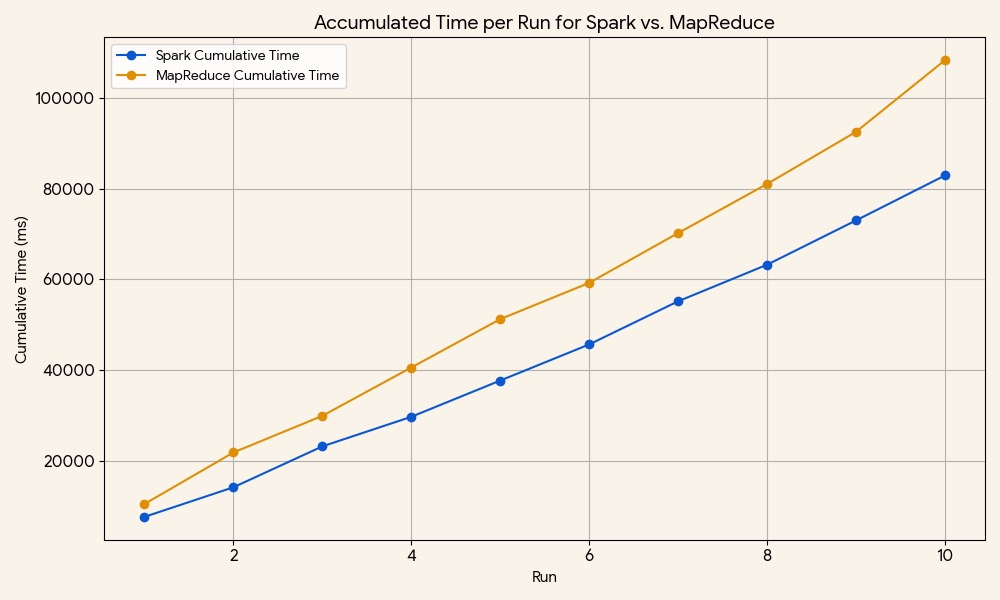
\includegraphics[width=\columnwidth]{img/MapReduce_vs_Spark.jpg}

\end{frame}

\begin{frame}[fragile]
    \frametitle{Performance Visualization}
    
    \begin{mycodetiny}
        # ========== MAPREDUCE ========== #
        Target B (ARFK...) was found 4 levels from Target A (ARO6...)
        It was connected to 3 artists at that level.
        Tracing path from B to A...
        Path found:
        ARO6... -> ARF6... -> ARIW... -> ARSO... -> ARFK...
        
        # ========== SPARK ========== #
        Target B (ARFK...) was found 4 levels from Target A (ARO6...) and was connected to 3 artists at that level.
        Path found:
        ARO6... -> ARF6... -> ARH6... -> ARBQ... -> ARFK...
    \end{mycodetiny}

    \centering
    \textit{Those are the results for both Spark and MapReduce, proving our point for algorithm consistency and data accuracy.}
\end{frame}

\begin{frame}[fragile]
    \frametitle{Summary}
    
    \begin{itemize}
        \item MapReduce: A powerful and robust tool for large-scale batch processing, especially for single-pass jobs.
        \item Spark: An ideal framework for iterative algorithms and machine learning, where in-memory caching provides a significant performance advantage.
        \item BFS Implementation: While both frameworks can solve the problem, Spark's architecture is fundamentally better suited for the iterative nature of BFS.
    \end{itemize}
\end{frame}

\section{Year Prediction}

\begin{frame}{Why Dimensionality Reduction? (PCA Motivation)}

\textbf{Correlation Analysis}
\begin{itemize}
    \item 64 numeric features per song
    \item \textbf{1569 out of 2016} pairs have correlation \textless{} 0.2
    \item \textbf{78\%} of pairs are weakly correlated
\end{itemize}

\textbf{Why it matters}
\begin{itemize}
    \item High dimensionality \rightarrow noise, redundancy, slower models
    \item PCA finds uncorrelated directions with most variance
\end{itemize}

\textbf{Result}
\begin{itemize}
    \item Reduced 64 features -> \textbf{32 components}
    \item Explained variance retained: \textbf{90\%+}
\end{itemize}

\end{frame}

\begin{frame}{Musical Features: Pitch and Timbre}

\textbf{Pitch}
\begin{itemize}
    \item What \textbf{notes} are used - C, D, E, ..., B
    \item Melody and harmony
    \item 12D vector (1 value per pitch class)
\end{itemize}

\textbf{Timbre}
\begin{itemize}
    \item \textbf{Texture} of sound - smooth, sharp, warm, bright
    \item Depends on instruments and production
    \item 12D vector from audio spectrum (e.g., MFCC)
\end{itemize}


\textbf{Why important?}
\begin{itemize}
    \item Pitch = \textbf{what is played}; Timbre = \textbf{how it sounds}
    \item Both change with time -> useful for predicting song year
\end{itemize}

\end{frame}

\begin{frame}{PCA Component Comparison (Linear Regression)}

\begin{itemize}
    \item Tested PCA with \textbf{k = 10, 32, 52} components
    \item Fewer components $\rightarrow$ worse performance:
    \begin{itemize}
        \item \textbf{R\textsuperscript{2}} dropped: 0.26 $\rightarrow$ 0.21 $\rightarrow$ 0.14 \\
              \small (how much variance is explained - higher is better)
        \item \textbf{RMSE} increased: 9.37 $\rightarrow$ 9.73 $\rightarrow$ 10.14 \\
              \small (average prediction error in years)
    \end{itemize}
    \item \textbf{k = 32} offers a good trade-off between performance and simplicity
    \item \textcolor{red}{Problem of having too many features: hard to fit a single linear model}
\end{itemize}

\end{frame}



\begin{frame}{Trying SGD for Linear Regression}

\textbf{Goal:}
\begin{itemize}
    \item Improve performance by switching to \textbf{SGD-based linear regression}
    \item Hope: increase R\textsuperscript{2} beyond previous baseline
\end{itemize}

\textbf{What we did:}
\begin{itemize}
    \item Used PCA (k = 32) and normalized target label (year)
    \item Tuned key hyperparameters:
    \begin{itemize}
        \item Learning rate, iterations, regularization
    \end{itemize}
\end{itemize}

\textbf{Result:}
\begin{itemize}
    \item \textbf{R\textsuperscript{2}} = 0.21 (on normalized labels)
\end{itemize}

\textcolor{red}{
Despite tuning, performance remained close to baseline.
\\
We reached the limitation of linear regression for this task.
}

\end{frame}


\begin{frame}{Logistic Regression for Year Classification}

\textbf{Goal:}
\begin{itemize}
    \item Frame year prediction as a \textbf{multi-class classification} task
    \item Train logistic regression using \textbf{PCA-32 features}
\end{itemize}

\textbf{Setup:}
\begin{itemize}
    \item Used pipeline: Assemble $\rightarrow$ Scale $\rightarrow$ PCA (k = 32)
    \item Tried different values for hyperparameters (e.g., \texttt{regParam}, \texttt{maxIter})
\end{itemize}

\textbf{Results:}
\begin{itemize}
    \item \textbf{Accuracy:} 9.7\%
\end{itemize}


\end{frame}




% \begin{frame}{Include a picture}

% \begin{columns}[T,onlytextwidth]

% 	\column{.4\halfwidth}
	
% 	\centering
% 	
\includegraphics[width=\columnwidth]{course}

% 	\column{1.6\halfwidth}

% 	\begin{example}

%     Two columns aligned to the top with a picture on the left and a citation.~\autocite{ece475}
	
%   \end{example}

% \end{columns}
		
% \end{frame}

\begin{frame}[fragile]
    \frametitle{Mini-batch Gradient Descent in sklearn}
    \textbf{First Attempt}
    \begin{itemize}
        \item Use MLPRegressor from sklearn to examine how well timbre feature performs on year prediction
    \end{itemize}
    
    \begin{mycodetiny}
        mlp = MLPRegressor(
            hidden_layer_sizes=(1024, 512, 512, 256, 256, 128, 64, 32),
            activation='relu',
            solver='adam',
            alpha=0.00001,
            batch_size=128,
            learning_rate='adaptive',
            early_stopping=True,
            validation_fraction=0.15,
            max_iter=1000,
            n_iter_no_change=20
        )
    \end{mycodetiny}
\end{frame}

\begin{frame}{Mini-batch Gradient Descent in sklearn}

\textbf{Outcome of MLPRegressor}
\begin{itemize}
    \item Mean Squared Error: 117.11
    \item Mean Absolute Error: 6.39 years
\end{itemize}
\end{frame}

\begin{frame}[fragile]
    \frametitle{{MLPRegressor}}
\begin{figure}
    \centering
    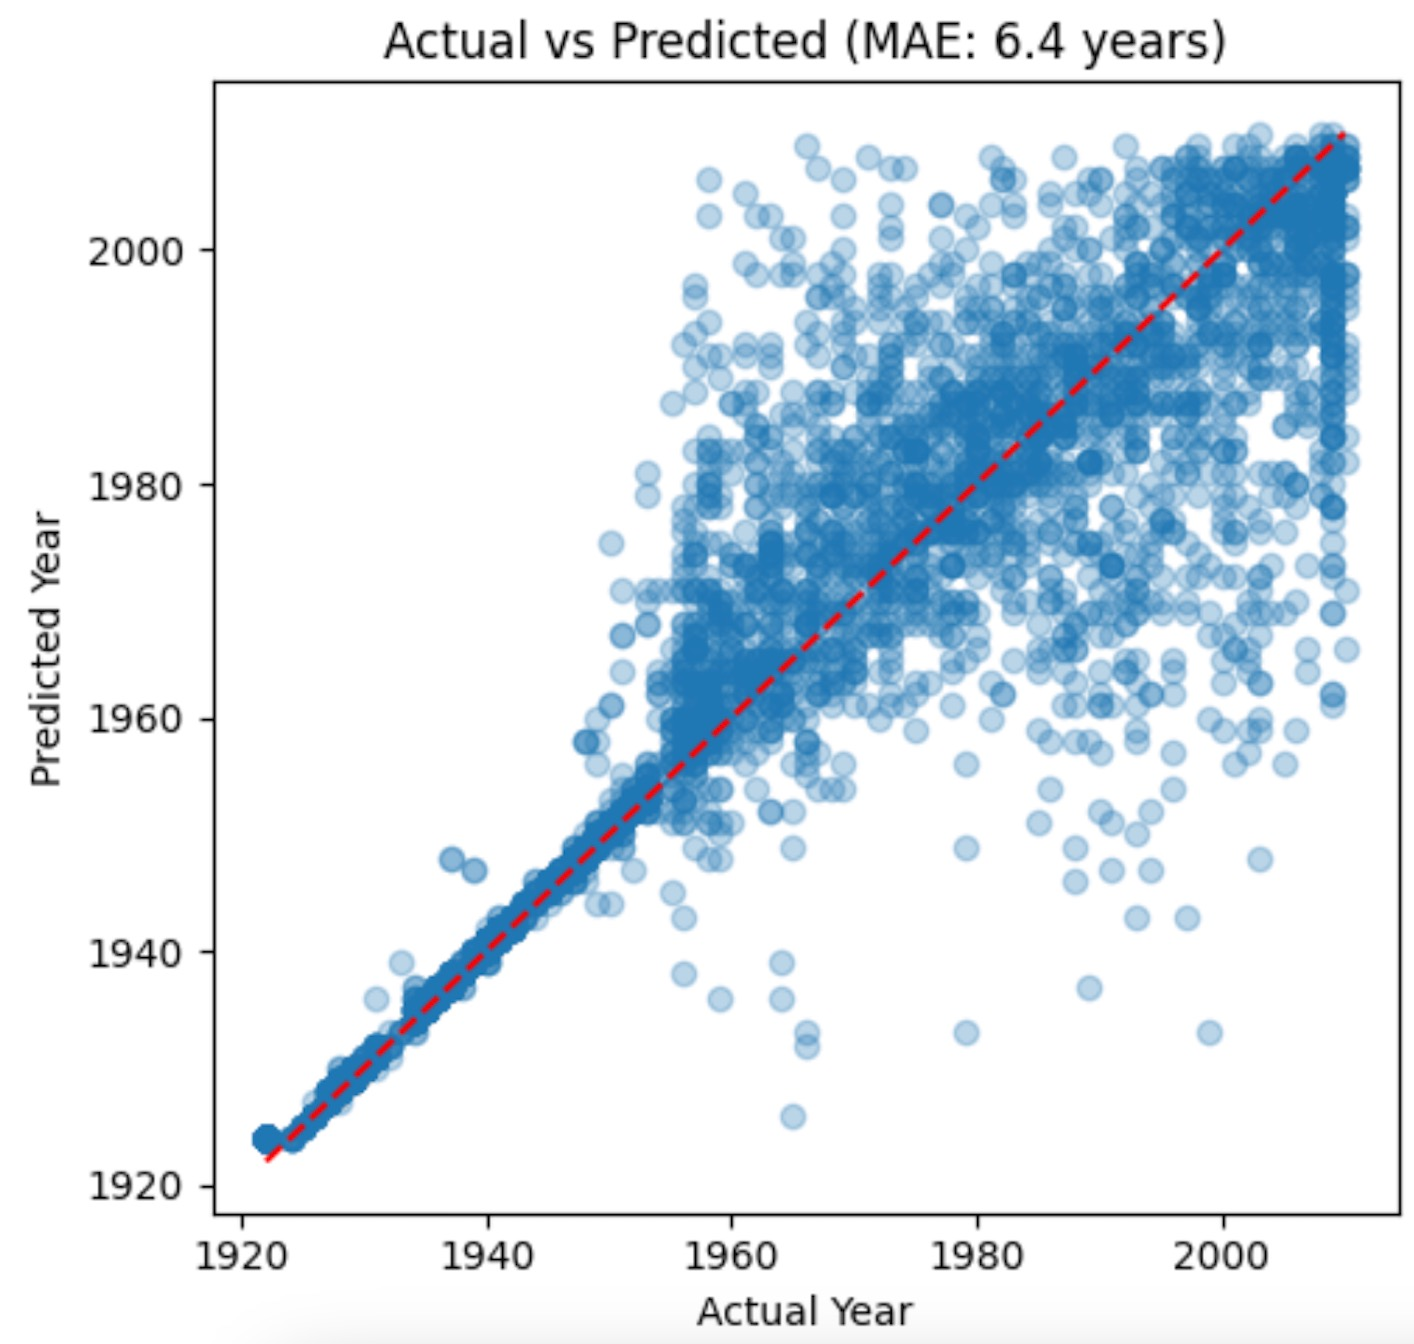
\includegraphics[width=0.75\linewidth]{img/actualVSpredicted.jpg}
\end{figure}
\end{frame}

\begin{frame}[fragile]
    \frametitle{{MLPRegressor}}
\begin{figure}
    \centering
    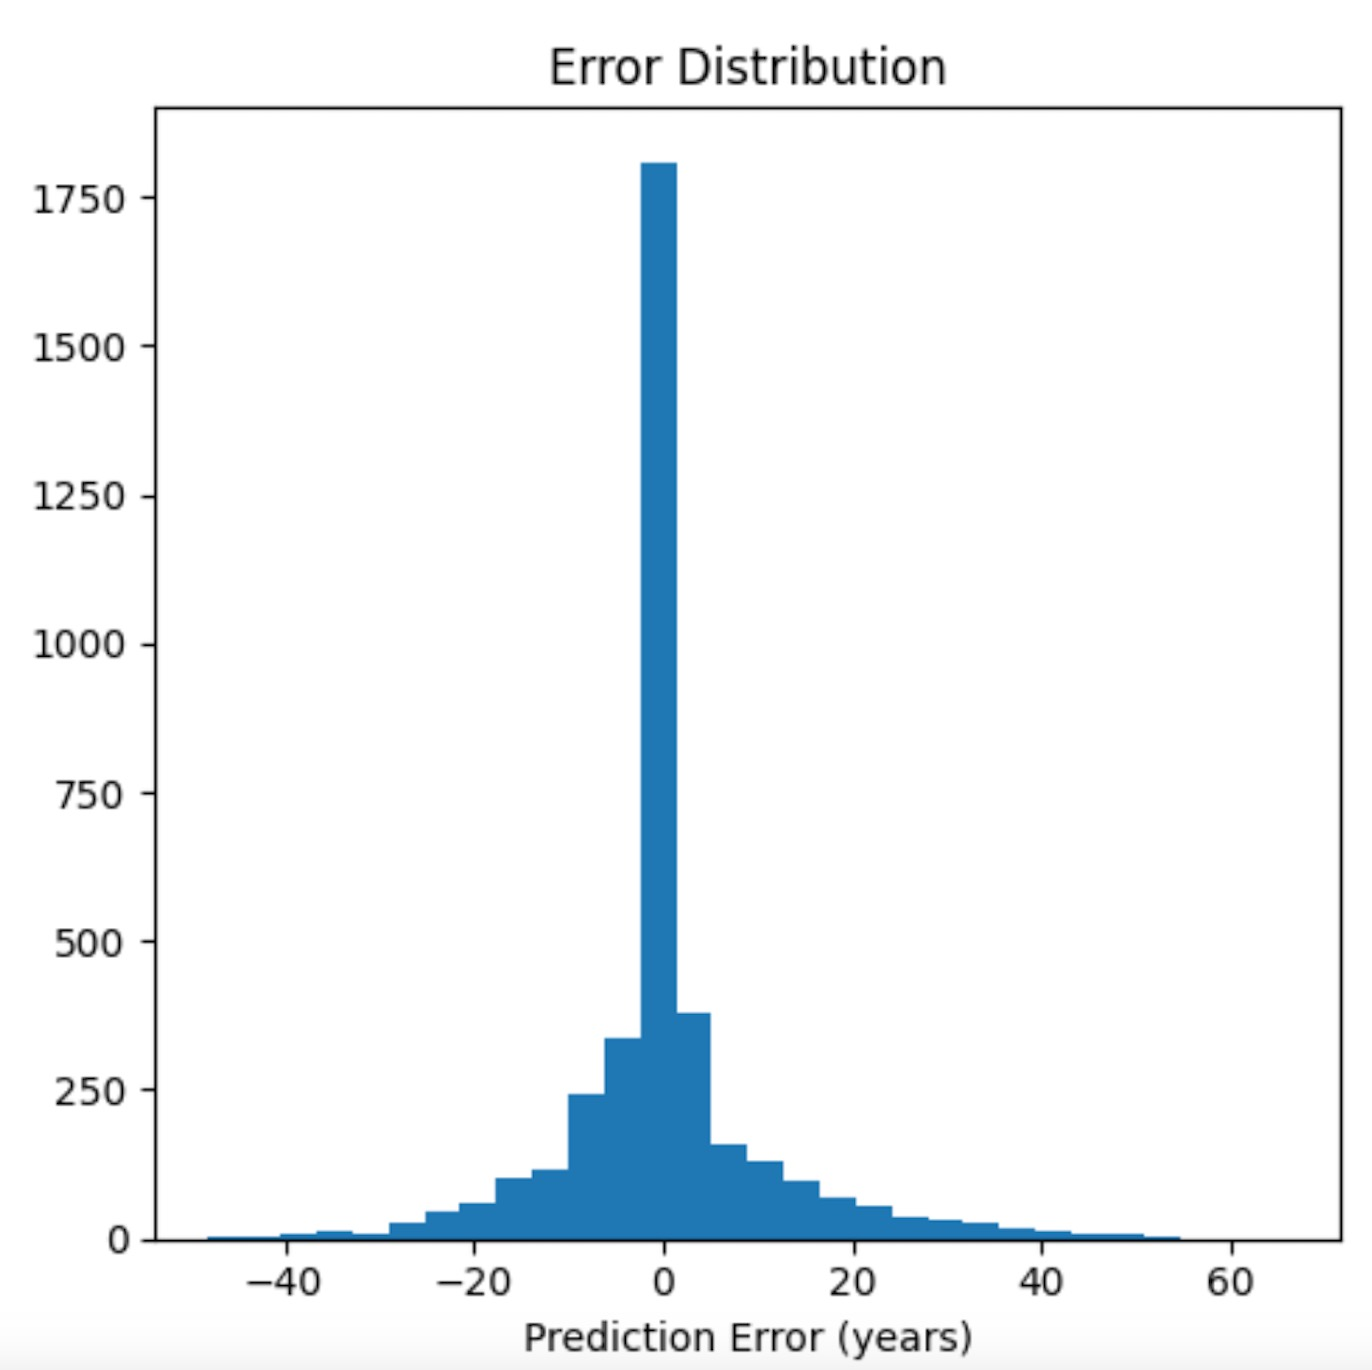
\includegraphics[width=0.7\linewidth]{img/errorDist.jpg}
\end{figure}
\end{frame}

\begin{frame}[fragile]
    \frametitle{{MLPRegressor}}
    \begin{center}
        It makes sense if we counts the samples in decades.

        Data Imbalance!
    \end{center}
\begin{figure}
    \centering
    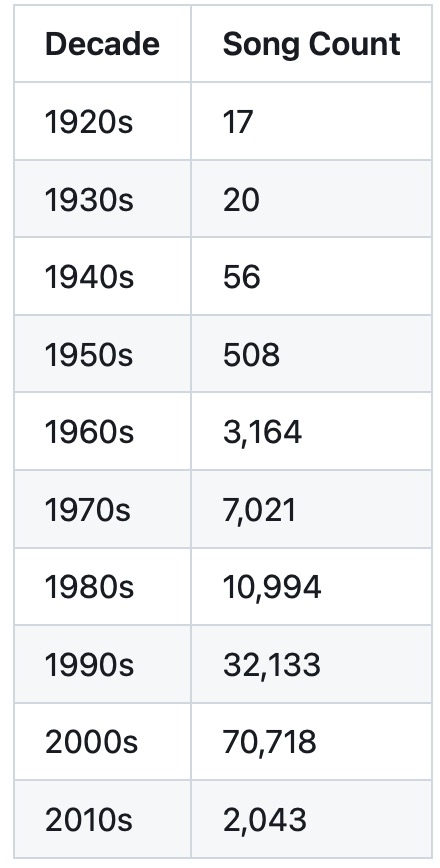
\includegraphics[width=0.3\linewidth]{img/decades.jpg}
\end{figure}
\end{frame}

\begin{frame}[fragile]
    \frametitle{{MLPRegressor}}
\begin{figure}
    \centering
    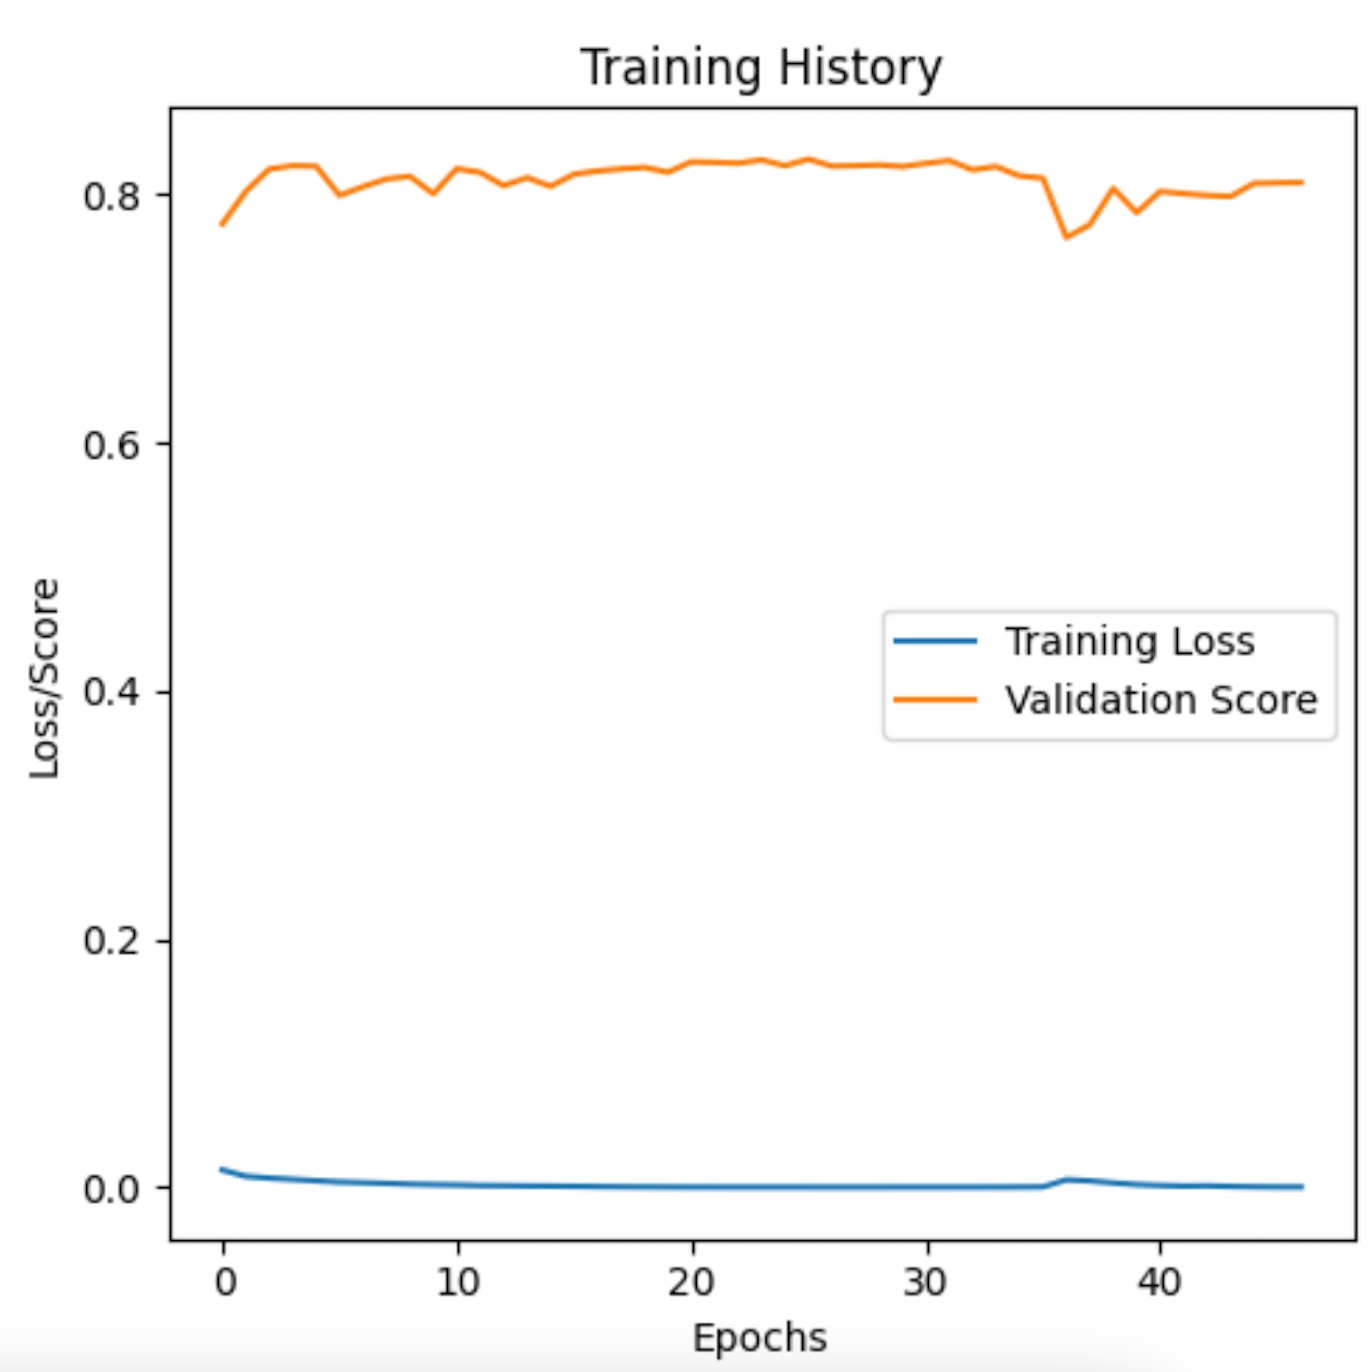
\includegraphics[width=0.7\linewidth]{img/trainHistory.jpg}
\end{figure}
\end{frame}

\begin{frame}[fragile]
    \frametitle{Mini-batch Gradient Descent in Spark}
    \textbf{FMRegressor}
    \begin{itemize}
        \item Extends linear regression by modeling pairwise feature interactions efficiently using factorized parameters. 
        \item Automatically detects relationships between features (e.g., how ``timbre\_1" and ``pitch\_3" jointly affect the year).
    \end{itemize}
    
    \begin{mycodetiny}
        regressor = FMRegressor(
            labelCol="year_scaled",
            featuresCol="pcaFeatures",
            factorSize=4,
            solver="adamW",
            miniBatchFraction=0.2,
            maxIter=400,
            stepSize=0.05,
            regParam=0.01,
            seed=42
        )
    \end{mycodetiny}
\end{frame}


\begin{frame}[fragile]
    \frametitle{Mini-batch Gradient Descent in Spark}
    \textbf{FMRegressor}
    \begin{itemize}
        \item Extends linear regression by modeling pairwise feature interactions efficiently using factorized parameters. 
        \item Automatically detects relationships between features (e.g., how ``timbre\_1" and ``pitch\_3" jointly affect the year).
    \end{itemize}
    
    \begin{mycodetiny}
        regressor = FMRegressor(
            labelCol="year_scaled",
            featuresCol="pcaFeatures",
            factorSize=4,
            solver="adamW",
            miniBatchFraction=0.2,
            maxIter=400,
            stepSize=0.05,
            regParam=0.01,
            seed=42
        )
    \end{mycodetiny}
\end{frame}

\begin{frame}{Mini-batch Gradient Descent in Spark}

\textbf{Outcome of FMRegressor}
\vspace{1cm}
\begin{multicols}{2}
\begin{enumerate}
    \item timbre
        \begin{itemize}
            \item RMSE: 10.82    
            \item MAE: 8.09 years
        \end{itemize}
    \columnbreak
    \item timbre + pitch
        \begin{itemize}
            \item 95\% variance PCA, k = 59
            \item RMSE: 10.32 
            \item MAE: 7.58 years
        \end{itemize}
\end{enumerate}
\end{multicols}
\begin{center}
    However, the current $R^2$ is too bad! ($R^2$ < 0.1 !).
    More architecture exploration will be needed.
\end{center}
\end{frame}

\begin{frame}[fragile]
    \frametitle{Linear Regressor in Spark}
    \textbf{LinearRegressor}
    \begin{itemize}
        \item Latest Spark recommend using LinearRegressor instead of LinearRegressorWithSGD. 
        \item \textbf{Model}: Linear Regression with Polynomial Features (degree=2)
        \item \textbf{Scaler}: RobustScaler (handles outliers better)
        \item \textbf{Optimizer}: L-BFGS (better convergence for small/medium datasets)
        \item \textbf{Balancing}: Stratified sampling (5-year bins, 1k samples per bin)
    \end{itemize}
    
    \begin{mycodetiny}
        lr = LinearRegression(
            featuresCol="polyFeatures",
            labelCol="year",
            solver="l-bfgs",
            maxIter=400,
            tol=1e-6
        )
    \end{mycodetiny}
\end{frame}

\begin{frame}{Linear Regressor in Spark}

\textbf{Outcome of LinearRegressor}
\begin{itemize}
    \item RMSE: 15.38
    \item MAE: 9.82 years
    \item $R^2$: 0.68
\end{itemize}
\end{frame}

\begin{frame}[fragile]
    \frametitle{{Linear Regressor in Spark}}
\begin{figure}
    \centering
    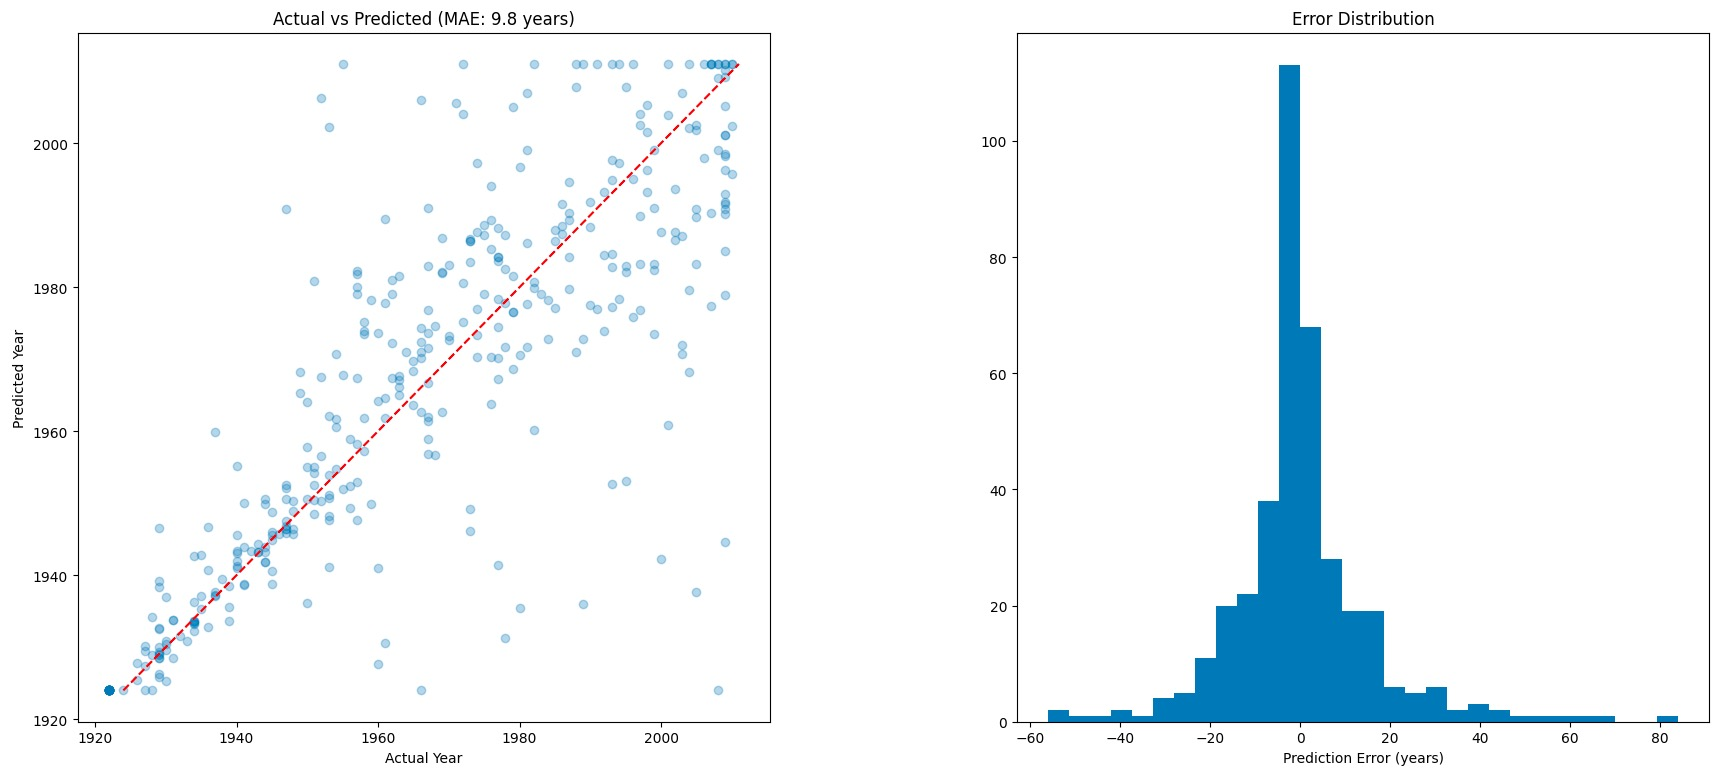
\includegraphics[width=1\linewidth]{img/Linear.jpg}
\end{figure}
\end{frame}

\begin{frame}{GBTRegressor in Spark}

\textbf{Outcome of GBTRegressor}
\begin{itemize}
    \item timbre
    \item RMSE: 9.60
    \item MAE: 6.89 years
    \item $R^2$: 0.20
\end{itemize}
\end{frame}
% \section{Bibliography}

% \begin{frame}[allowframebreaks]{References}

%     \printbibliography[heading=none]

% \end{frame}

\thankframe

\end{document}
